\modeCorrection

\renewcommand{\thesubsection}{\textcolor{red}{\Roman{section}.\arabic{subsection}}}
\renewcommand{\thesubsubsection}{\textcolor{red}{\Roman{section}.\arabic{subsection}.\alph{subsubsection}}}

\setcounter{section}{0}
\setcounter{document}{0}
\enTeteAct{6 : De l'espèce chimique à l'entité : la mole}{1}{Dénombrer les entités dans le basilic}

\begin{center}
\begin{mdframed}[style=titr, leftmargin=60pt, rightmargin=60pt, innertopmargin=7pt, innerbottommargin=7pt, innerrightmargin=8pt, innerleftmargin=8pt]

\begin{center}
\large{\textbf{Activité documentaire : Dénombrer les entités dans le basilic}}
\end{center}

\end{mdframed}
\end{center}

\begin{tcolorbox}[colback=orange!5!white,colframe=orange!75!black,title= Contexte de l'activité]
\begin{minipage}{0.7\textwidth}
    La matière est constitué d'entités chimiques invisibles à l'\oe il nu mais il est quand même possible de les visualiser avec un microscope ! On peut même les manipuler un par un ! La société IBM a réussi à le faire en 2012 et à en faire un film :
    \begin{center}
        \url{https://ladigitale.dev/digiview/#/v/65a178ec87ac7}
    \end{center}

\end{minipage}
\begin{minipage}{0.25\textwidth}
    \begin{center}
        
\includegraphics[scale=0.3]{Images/Qrcode_IBM.png}
    \end{center}
\end{minipage}
\vspace{1cm}
\problematique{Peut-on dénombrer le nombre d'entités chimiques présentes dans une espèce chimique ?}
\end{tcolorbox}

\begin{tcolorbox}[colback=blue!5!white,colframe=blue!75!black,title=Objectifs :]
\begin{itemize}
    \item Utiliser le terme adapté parmi molécule, atome, anion, cation pour qualifier une entité chimique à partir d'une formule chimique donnée ;
    \item Définir une espèce chimique comme une collection d'un nombre très élevé d'entités identiques ;
    \item Travailler les puissances de 10 ;
\end{itemize}
\end{tcolorbox}

%\begin{mdframed}[style=autreexo]
%\textbf{\bsc{Consignes :}}
%\begin{itemize}
%    \item Lever la main si vous souhaitez vous déplacer,
%    \item Lever la main si vous souhaitez un indice,
%    \item Vous pouvez travailler en binôme \textbf{\underline{uniquement}} avec votre voisin de table,
 %   \item Vous pouvez rendre le travail à la fin de l'heure si vous améliorer votre note d'interrogation.
   
%\end{itemize}
%\end{mdframed}

\begin{minipage}{0.5\textwidth}
    \begin{doc}{Le basilic, une plante aromatique}
        \begin{center}
            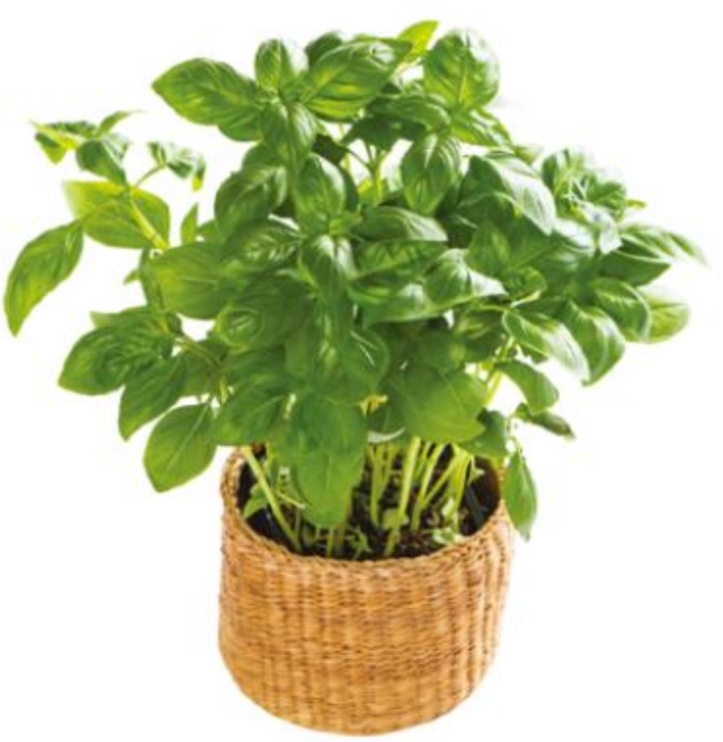
\includegraphics[scale=0.5]{Images/basilic.PNG}
        \end{center}
    \end{doc}
\end{minipage}
\begin{minipage}{0.5\textwidth}
\begin{doc}{Composition du basilic pour 100g}
     \begin{center}
        \begin{tabular}{|c|c|}
        \hline
             \cellcolor{blue!25} Espèces & \cellcolor{blue!25} Masse pour 100g  \\
        \hline
             Eau \chemform{H_2O} & 90,8g \\
        \hline
             Ion calcium \chemform{Ca^{2+}} & 273~mg\\
        \hline
             Acide oléique \chemform{C_{18}H_{34}O_2} & 0,09~g\\
        \hline
            Vitamine A \chemform{C_{20}H_{30}O} & 523~$\mu$g\\
        \hline 
            Autres & 8,84~g \\
        \hline
        \end{tabular}
    \end{center}
\end{doc}
\end{minipage}
\newpage
\begin{doc}{Détermination de la masse d'une molécule ou d'un ion polyatomique}
\vspace{-1.5cm}
    \begin{tcolorbox}[colback=red!5!white,colframe=red!75!black,title=\textbf{Règle sur les molécules et les ions polyatomiques : }]
\begin{itemize}[label=\textbullet, font=\large]
    \item La masse d'une molécule se calcule en faisant la somme des masses de chacun des atomes la constituant. Exemple pour le glucose de formule chimique \chemform{C_6H_{12}O_6} : 
        \begin{equation*}
            m(\text{\chemform{C_6H_{12}O_6}}) = 6\times m(C) + 12\times m(H) + 6\times m(O)
        \end{equation*}
    \item C'est la même règle pour déterminer la masse d'un ion polyatomique. Exemple pour l'ion sulfate de formule chimique \chemform{SO_4}$^{2-}$ :
        \begin{equation*}
            m(\text{\chemform{SO_4}$^{2-}$}) = 1\times m(S) + 4\times m(O)
        \end{equation*}
\end{itemize}
\end{tcolorbox}
\end{doc}
\begin{minipage}{0.4\textwidth}
    \begin{doc}{Masse de quelques entités chimiques}
\vspace{-1cm}
\begin{align*}
    m(\text{H}) &= 1,67\times10^{-27}~\text{kg} \\  m(\text{C}) &= 1,99\times10^{-26}~\text{kg} \\
    m(\text{O}) &= 2,66\times10^{-26}~\text{kg} \\ m(\text{Ca$^{2+}$}) &= 6,66\times10^{-26}~\text{kg} 
\end{align*}
\end{doc}
\end{minipage}
\begin{minipage}{0.6\textwidth}
\begin{doc}{Modèle moléculaire de l'acide oléique}
\vspace{-1cm}
\begin{center}
    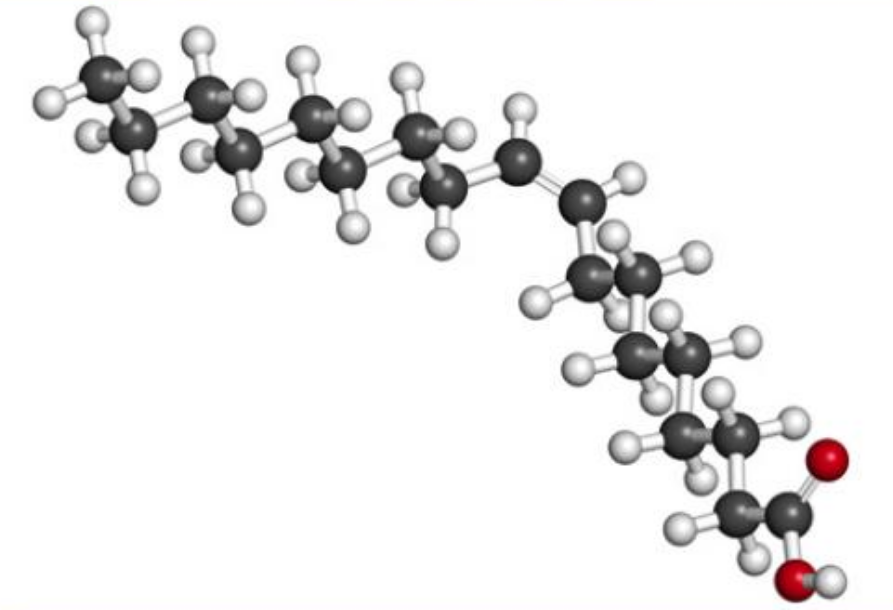
\includegraphics[scale=0.4]{Images/Modele_moleculaire_acideoleique.PNG}
\end{center}
\end{doc}    
\end{minipage}
\vspace{0.5cm}
\renewcommand{\arraystretch}{1.5}
\question{\`{A} l'aide du document 2, classer les quatre constituants du basilic donnés selon la nature des entités qui les constituent (atomique, ionique moléculaire) : 
\begin{center}
        \begin{tabular}{|C{0.31}|C{0.31}|C{0.31}|}
        \hline
             \cellcolor{orange!25} Atomique & \cellcolor{orange!25}Moléculaire & \cellcolor{orange!25} Ionique \\ 
            \hline
             & & \\
             \hline
        \end{tabular}
\end{center}
}
{\begin{center}
    \begin{tabular}{|C{0.31}|C{0.31}|C{0.31}|}
        \hline
        \cellcolor{orange!25} Atomique & \cellcolor{orange!25}Moléculaire & \cellcolor{orange!25} Ionique \\ 
        \hline
        & Eau, acide oléique, Vitamine A & Ion calcium Ca$^{2}$\\
        \hline
        \end{tabular}
\end{center}}{0}

\question{\`{A} l'aide du document 2 et 5, déterminer le nombre d'atomes de carbone, d'oxygène et d'hydrogène dans l'acide oléique. \newline\texteTrouMultiLignes{~}{3}}{Les indices correspondent aux nombre d'atomes présents dans la molécule : il y a donc 6 atomes de carbone, 34 atomes d'hydrogène et 2 atomes d'oxygène.}{0}
\\
\question{En vous aidant des règles du document 3, calculer la masse d'une seule entité pour chacune des espèces chimiques du basilic. \newline\texteTrouMultiLignes{~}{15}}{
\begin{itemize}
    \item Pour l'eau \chemform{H_2O} : $m(\text{\chemform{H_2O}})=m(O)+2\times m(H) = 1\times 2,66\times10^{-26} + 2\times 1,67\times10^{-27} = 2,99\times10^{-26}$~kg ;
    \item Pour l'ion calcium \chemform{Ca^+} : $m(\text{\chemform{Ca^{2+}}}) = m(Ca) = 6,66\times10^{-26}$~kg ;
    \item Pour l'acide oléique \chemform{C_{18}H_{34}O_2} :
    $m(\text{\chemform{C_{18}H_{34}O_2}}) = 18\times m(C) + 34\times m(H) + 2\times m(O) = 46,8\times10^{-26}$~kg ;
    \item Pour la vitamine A \chemform{C_{20}H_{30}O} : $m(\text{\chemform{C_{20}H_{30}O}}) = 20\times m(C) + 30\times m(H) + 2\times m(O) = 47,5\times10^{-26}$~kg ;
\end{itemize}
}{0}
%\\
\question{Déterminer le nombre de ces entités dans 100~g de basilic. \newline\texteTrouMultiLignes{~}{10}}{Le nombre d'une entité peut être calculé comme la masse totale de l'entité présente dans le basilic pour 100~g divisé par la masse d'une entité. Donc :
\begin{itemize}
    \item Pour l'eau \chemform{H_2O} : $N(\text{\chemform{H_2O}}) = \frac{m(\text{\chemform{H_2O},basilic})}{m(\text{\chemform{H_2O}})} = \frac{90,8\times10^{-3}~\text{kg}}{2,99\times10^{-26}~\text{kg}} = 30,4\times10^{23}$ molécules d'eau dans 100g de basilic ;
    \item Pour l'ion calcium \chemform{Ca^+} : $N(\text{\chemform{Ca^{2+}}}) = \frac{m(\text{\chemform{Ca^{2+}},basilic})}{m(\text{\chemform{Ca^{2+}}})} = 4,10\times10^{21}$ ions calcium dans 100g de basilic ;
    \item Pour l'acide oléique \chemform{C_{18}H_{34}O_2} :    $N(\text{\chemform{C_{18}H_{34}O_2}})= \frac{m(\text{\chemform{C_{18}H_{34}O_2},basilic})}{m(\text{\chemform{C_{18}H_{34}O_2}})} = 1,92\times10^{20}$ molécules d'acide oléique dans 100g de basilic ;
    \item Pour la vitamine A \chemform{C_{20}H_{30}O} : $N(\text{\chemform{C_{20}H_{30}O}}) = \frac{m(\text{\chemform{C_{20}H_{30}O},basilic})}{m(\text{\chemform{C_{20}H_{30}O}})} = 1,86\times10^{22}$ molécules de vitamine A dans 100g de basilic ;
\end{itemize}
}{0}


\begin{difficile}{Bilan de l'activité}
%\vspace{18cm}
Il existe une énorme quantité d'entités chimiques dans la matière à notre échelle ! Il est impossible de donner du sens à ces nombres pour le cerveau humain. D'autre part, le calcul est laborieux et relativement compliquer à réaliser.\\
Plutôt que de travailler avec les entités chimiques, le chimiste va plutôt les rassembler en \og paquets \fg~ d'un très grand nombre de particules. Un paquet est appelé \og \textcolor{red}{mole} \fg.\\
Soit N le nombre d'entités chimiques présentes et n le nombre de mole de cette entité présente dans une espèce chimique. Alors :
\begin{empheq}[box=\fbox]{equation*}
    \mathrm{N} = n\times\mathrm{N_A}
\end{empheq}
où :
\begin{empheq}[box=\fbox]{equation*}
    \mathrm{N_A} = 6,022\times10^{23}\text{mol$^{-1}$}
\end{empheq}
est appelé \textcolor{red}{constante d'Avogadro}. Cette constante représente le nombre d'entités chimiques par mole d'entité. Cette constante fait donc le lien entre l'échelle microscopique (l'entité) et l'échelle macroscopique (l'espèce chimique = collection d'un grand nombre d'entité).
\end{difficile}